\section{Penyajian Data Uji Coba}

Pada penelitian ini dilakukan uji coba menggunakan data lokasi seluruh SMA di Kabupaten Probolinggo, dan dijalankan menggunakan python. Berikut adalah sajian data hasil uji coba.

\subsection{Pengambilan Data Lokasi}

Data yang digunakan adalah data koordinat lokasi yang diekspor melalui google earth. Pengujian Pengambilan data lokasi bertujuan untuk menunjukkan bahwa sistem 
mampu membaca input yang dimasukkan. Dapat dilihat pada Lampiran \ref{lampiran1} seluruh nama-nama SMA di Kabupaten Probolinggo beserta koordinat lokasinya. Visualisasi data dari koordinat-koordinat SMA di kabupaten probolinggo dapat dilihat pada Gambar \ref{fig:petasma}.

\begin{figure}[h!]
  \centering
  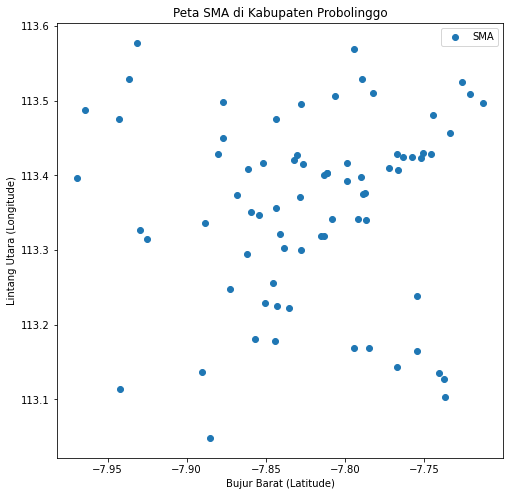
\includegraphics[width=0.5\textwidth]{peta sma.png}
  \caption{Visualisasi lokasi SMA di Kabupaten Probolinggo}
  \label{fig:petasma}
\end{figure}

Setelah mendapatkan lokasi yang akan diproses, selanjutnya adalah menentukan beberapa titik centroid secara random, dalam penelitian ini akan diambil 7 centroid secara random seperti pada Tabel \ref{tab:dasen} dan \ref{fig:visdasen}.

\begin{table}[H]
\centering
\begin{tabular}{cccll}
\cellcolor[HTML]{4472C4}{\color[HTML]{FFFFFF} \textbf{Nama   Centroid}} & \cellcolor[HTML]{4472C4}{\color[HTML]{FFFFFF} \textbf{Latitude (Sumbu X)}} & \cellcolor[HTML]{4472C4}{\color[HTML]{FFFFFF} \textbf{Longitude (Sumbu Y)}} &  &  \\
\cellcolor[HTML]{D9E1F2}A                                               & \cellcolor[HTML]{D9E1F2}-7,81                                              & \cellcolor[HTML]{D9E1F2}113,14                                              &  &  \\
B                                                                       & -7,77                                                                      & 113,51                                                                      &  &  \\
\cellcolor[HTML]{D9E1F2}C                                               & \cellcolor[HTML]{D9E1F2}-7,77                                              & \cellcolor[HTML]{D9E1F2}113,40                                              &  &  \\
D                                                                       & -7,88                                                                      & 113,35                                                                      &  &  \\
\cellcolor[HTML]{D9E1F2}E                                               & \cellcolor[HTML]{D9E1F2}-7,93                                              & \cellcolor[HTML]{D9E1F2}113,51                                              &  &  \\
F                                                                       & -7,83                                                                      & 113,27                                                                      &  &  \\
\cellcolor[HTML]{D9E1F2}G                                               & \cellcolor[HTML]{D9E1F2}-7,84                                              & \cellcolor[HTML]{D9E1F2}113,42                                              &  & 
\end{tabular}
\caption{Koordinat titik-titik centroid pada pembagian menjadi 8 klaster}
\label{tab:dasen}
\end{table}

\begin{figure}[h!]
	\centering
	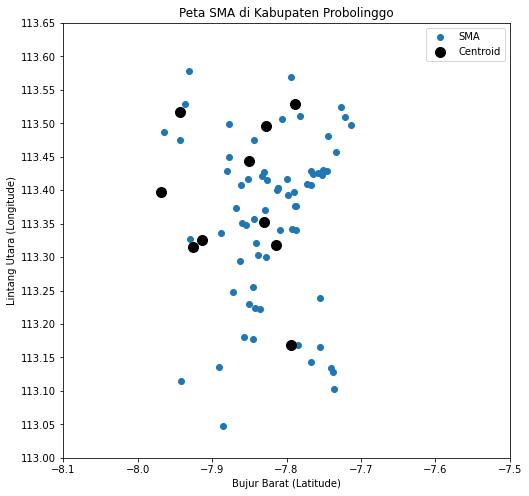
\includegraphics[width=0.5\textwidth]{titik centroid.png}
	\caption{Visualisasi Centroid}
	\label{fig:visdasen}
\end{figure}

\subsection{Proses Pengklasteran Data}

Pada tahap ini metode yang digunakan adalah metode $K-$means untuk mengklaster data. Langkah-langkah nya adalah sebagai berikut.

\begin{enumerate}
	\item Menentukan jumlah klaster, dalam hal ini yang digunakan adalah 7 klaster.
	\item Memilih titik-titik centroid sebanyak jumlah klaster seperti pada Tabel \ref{tab:dasen} dan \ref{fig:visdasen}
	\item \label{ulang3} Hitung jarak tiap titik sekolah yang ada dengan masing-masing \textit{centroid}. Penghitungan jarak menggunakan \textit{Euclidean Distance} pada persamaan (\ref{eq:euclidean3}.
	\item Kelompokan data ke dalam klaster yang memiliki jarak paling minimum.
	\item Setelah seluruh titik sekolah masuk ke dalam klaster-klaster, hitung \textit{centroid} yang baru dengan cara menghitung rata-rata titik sekolah yang ada di dalam klaster tersebut. Lakukan hal yang sama pada klaster yang lain.
	\item Jika terdapat perubahan klaster, maka ulangi langkah \ref{ulang3} hingga tidak ada perubahan anggota pada tiap klaster. Jika \textit{centroid} yang baru tidak berubah dari sebelumnya, maka proses berhenti, karena \textit{centroid} yang tidak berubah menyebabkan anggota klaster juga tidak berubah.
	
	\begin{equation}
	\left[ \left( x,y \right) ,\left( a,b \right)\right]=\sqrt{\left( x-a \right)^{2}+\left( y-b \right)^{2}}
	\label{eq:euclidean3}
	\end{equation}
	
	\item Setelah semua data terklasifikasi, selanjutnya adalah memperbarui titik-titik centroid dengan cara menghitung rata-rata tiap anggota klaster.
\end{enumerate}

\subsection{Proses TSP menggunakan Algoritma Genetika}

Setelah data terklaster seperti pada Gambar \ref{fig:hasilklas} selanjutnya adalah mencari rute terdekatnya menggunakan Algoritma Genetika

\begin{figure}[h!]
	\centering
	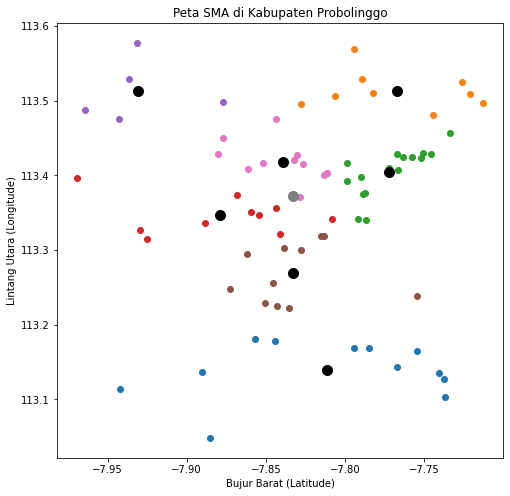
\includegraphics[width=0.5\textwidth]{hasil klaster.png}
	\caption{Visualisasi klaster sesuai warna}
	\label{fig:hasilklas}
\end{figure}

\begin{enumerate}
	\item Bangkitkan beberapa populasi awal berisi sejumlah kromosom yang di dalamnya terdapat urutan perjalanan menuju titik sekolah.
	\item \label{ulang4} Hitung nilai \textit{fitness} (total jarak) dari tiap kromosom.
	\item Menetapkan probabilitas \textit{crossover} ($p_c$) dalam hal ini yang digunakan adalah $p_c=0,95$. Bangkitkan bilangan random (0,0000 sampai 1,0000) pada setiap kromosom, kromosom dengan bilangan random kurang dari $p_c$ maka akan dilakukan \textit{crossover}. Jika kromosom hasil \textit{crossover} memiliki \textit{fitness} yang lebih baik  dari kromosom awal, maka kromosom awal digantikan oleh kromosom hasil \textit{crossover}.
	\item Menetapkan probabilitas mutasi ($p_m$), dalam hal ini digunakan $p_m=0,1$. Bangkitakan bilangan random (0,0000 sampai 1,0000) pada setiap kromosom, kromosom yang memiliki bilangan random kuran dari $p_m$ maka akan dilakukan mutasi. Jika kromosom hasil mutasi memiliki \textit{fitness} yang lebih baik dari kromosom awal, maka kromosom awal digantikan oleh kromosom hasil mutasi.
	\item Jika hasil kurang optimal, iterasi dilakukan dengan cara kembali ke tahapan (\ref{ulang4}) untuk generasi berikutnya sampai hasil yang dilakukan optimal atau mendekati optimal.
\end{enumerate}

\subsection{Hasil dari proses \textbf{$k$}-means dan Algoritma Genetika}

Dari serangkaian proses di atas, menghasilkan beberapa rute optimal yang dapat dilalui seperti pada Gambar \ref{fig:vishasilmtsp}. Rute-rute yang dihasilkan telah diurutkan sebelumnya dan telah diekspor ke bentuk spreadsheet sehingga mempermudah pengguna dalam membaca data seperti pada Tabel \ref{tab:datahasil} merupakan urutan perjalanan pada klaster A.

\begin{figure}[h!]
	\centering
	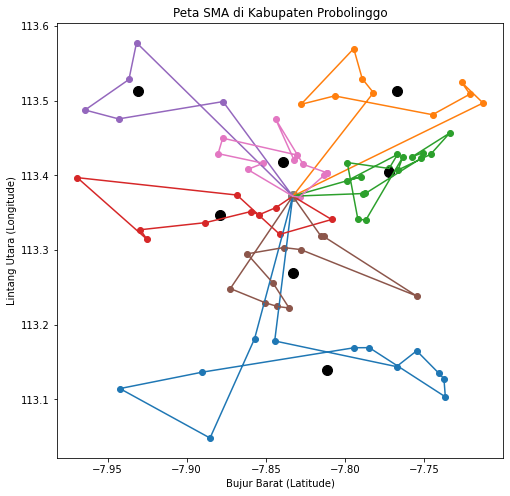
\includegraphics[width=0.5\textwidth]{hasil mtsp.png}
	\caption{Visualisasi hasil pembagian klaster dan rute yang dapat dilalui}
	\label{fig:vishasilmtsp}
\end{figure}

\begin{table}[h!]
\begin{adjustbox}{width=\columnwidth,center}
\begin{tabular}{lllcl}
\rowcolor[HTML]{4472C4} 
\multicolumn{1}{c}{\cellcolor[HTML]{4472C4}{\color[HTML]{FFFFFF} \textbf{Nama   Sekolah}}} & \multicolumn{1}{c}{\cellcolor[HTML]{4472C4}{\color[HTML]{FFFFFF} \textbf{Latitude (Sumbu X)}}} & \multicolumn{1}{c}{\cellcolor[HTML]{4472C4}{\color[HTML]{FFFFFF} \textbf{Longitude (Sumbu Y)}}} & {\color[HTML]{FFFFFF} \textbf{Klaster}} & \multicolumn{1}{c}{\cellcolor[HTML]{4472C4}{\color[HTML]{FFFFFF} \textbf{Urutan}}} \\
\rowcolor[HTML]{D9E1F2} 
SMAS ISLAM MIFTAHUL ARIFIN                                                                 & -7,86                                                                                          & 113,18                                                                                          & A                                       & 0                                                                                  \\
SMAN   1 SUKAPURA                                                                          & -7,89                                                                                          & 113,05                                                                                          & A                                       & 1                                                                                  \\
\rowcolor[HTML]{D9E1F2} 
SMAN 1 SUMBER                                                                              & -7,94                                                                                          & 113,11                                                                                          & A                                       & 2                                                                                  \\
SMA   NEGERI 1 KURIPAN                                                                     & -7,89                                                                                          & 113,14                                                                                          & A                                       & 3                                                                                  \\
\rowcolor[HTML]{D9E1F2} 
SMAS ISLAM SUMBERASIH                                                                      & -7,79                                                                                          & 113,17                                                                                          & A                                       & 4                                                                                  \\
SMAS   WALI SONGO                                                                          & -7,78                                                                                          & 113,17                                                                                          & A                                       & 5                                                                                  \\
\rowcolor[HTML]{D9E1F2} 
SMAN 1 TONGAS                                                                              & -7,74                                                                                          & 113,10                                                                                          & A                                       & 6                                                                                  \\
SMAS   ISLAM TAJUNG SARI                                                                   & -7,74                                                                                          & 113,13                                                                                          & A                                       & 7                                                                                  \\
\rowcolor[HTML]{D9E1F2} 
SMA NEGERI 1 SUMBERASIH                                                                    & -7,74                                                                                          & 113,13                                                                                          & A                                       & 8                                                                                  \\
SMAS   ASSUBHAN                                                                            & -7,75                                                                                          & 113,16                                                                                          & A                                       & 9                                                                                  \\
\rowcolor[HTML]{D9E1F2} 
SMAS DARUL AKHLAQ                                                                          & -7,77                                                                                          & 113,14                                                                                          & A                                       & 10                                                                                 \\
SMAN   1 BANTARAN                                                                          & -7,84                                                                                          & 113,18                                                                                          & A                                       & 11                                                                                
\end{tabular}
\end{adjustbox}
\caption{Urutan perjalanan pada klaster A}
\label{tab:datahasil}
\end{table}